\documentclass[a4paper]{article} 
\addtolength{\hoffset}{-2.25cm}
\addtolength{\textwidth}{4.5cm}
\addtolength{\voffset}{-3.25cm}
\addtolength{\textheight}{5cm}
\setlength{\parskip}{0pt}
\setlength{\parindent}{0in}

%----------------------------------------------------------------------------------------
%	PACKAGES AND OTHER DOCUMENT CONFIGURATIONS
%----------------------------------------------------------------------------------------
\usepackage{bm} % Bold math symbols, !must be loaded before unicode-math!
\usepackage{blindtext} % Package to generate dummy text
\usepackage{enumerate} % Enumerate with redefinable labels
\usepackage{enumitem} % Enumerate with redefinable labels
\renewcommand{\thesubsection}{\thesection.\alph{subsection}} % Enumerate subsections with letters
\renewcommand{\thesubsubsection}{\thesubsection.\roman{subsubsection}} % Enumerate subsubsections with roman numerals
\usepackage{charter} % Use the Charter font
\usepackage[utf8]{inputenc} % Use UTF-8 encoding
\usepackage{microtype} % Slightly tweak font spacing for aesthetics
\usepackage[english, ngerman]{babel} % Language hyphenation and typographical rules
\usepackage{amsthm, amsmath, amssymb} % Mathematical typesetting
\newcommand{\argmax}[1]{\underset{#1}{\text{arg max}}\;}
\newcommand{\argmin}[1]{\underset{#1}{\text{arg min}}\;}
\newcommand{\mb}[1]{\mathbf{#1}}  % Bold math symbols shorthand
\usepackage{float} % Improved interface for floating objects
\usepackage[final, colorlinks = true, 
            linkcolor = black, 
            citecolor = black]{hyperref} % For hyperlinks in the PDF
\usepackage{graphicx, multicol} % Enhanced support for graphics
\usepackage{xcolor} % Driver-independent color extensions
\usepackage{marvosym, wasysym} % More symbols
\usepackage{rotating} % Rotation tools
\usepackage{censor} % Facilities for controlling restricted text
\usepackage{listings, style/lstlisting} % Environment for non-formatted code, !uses style file!
\usepackage{pseudocode} % Environment for specifying algorithms in a natural way
\usepackage{style/avm} % Environment for f-structures, !uses style file!
\usepackage{booktabs} % Enhances quality of tables
\usepackage{tikz-qtree} % Easy tree drawing tool
\usepackage{todonotes} % Tool to insert TODOs
\tikzset{every tree node/.style={align=center,anchor=north},
         level distance=2cm} % Configuration for q-trees
\usepackage{style/btree} % Configuration for b-trees and b+-trees, !uses style file!
\usepackage[backend=biber,style=numeric,
            sorting=nyt]{biblatex} % Complete reimplementation of bibliographic facilities
% \addbibresource{ecl.bib}
\usepackage{csquotes} % Context sensitive quotation facilities
\usepackage[yyyymmdd]{datetime} % Uses YEAR-MONTH-DAY format for dates
\renewcommand{\dateseparator}{-} % Sets dateseparator to '-'
\usepackage{fancyhdr} % Headers and footers
\pagestyle{fancy} % All pages have headers and footers
\fancyhead{}\renewcommand{\headrulewidth}{0pt} % Blank out the default header
\fancyfoot[L]{} % Custom footer text
\fancyfoot[C]{} % Custom footer text
\fancyfoot[R]{\thepage} % Custom footer text
\newcommand{\note}[1]{\marginpar{\scriptsize \textcolor{red}{#1}}} % Enables comments in red on margin
\newcommand{\iverson}[1]{\ensuremath{[#1]}} % Enables Iverson brackets
%----------------------------------------------------------------------------------------

\begin{document}

%-------------------------------
%	TITLE SECTION
%-------------------------------

\fancyhead[C]{}
\hrule \medskip % Upper rule
\begin{minipage}{0.295\textwidth} 
\raggedright
\footnotesize
Ryan Ott \hfill\\   
14862565 \hfill\\
ryan.ott@student.uva.nl
\end{minipage}
\begin{minipage}{0.4\textwidth} 
\centering 
\large 
Practical Assignment 2\\ 
\normalsize 
Deep Learning 1\\ 
\end{minipage}
\begin{minipage}{0.295\textwidth} 
\raggedleft
\today\hfill\\
\end{minipage}
\medskip\hrule 
\bigskip

%-------------------------------
%	CONTENTS
%-------------------------------

\section{Transfer Learning}
\subsection{Comparing Models}
\subsubsection{Inference Speed per Image against Accuracy and Number of Parameters}
With a Pearson correlation coefficient of 0.85 there seems to be a strong positive linear correlation between the
top-1 accuracy and the inference speed. The ViT-B/32 model performs best overall with a higher accuracy for its
inference speed than the trend suggests. Shown in Figure \ref{fig:Top1Acc-vs-Inference}.
\begin{figure}[h]
    \centering
    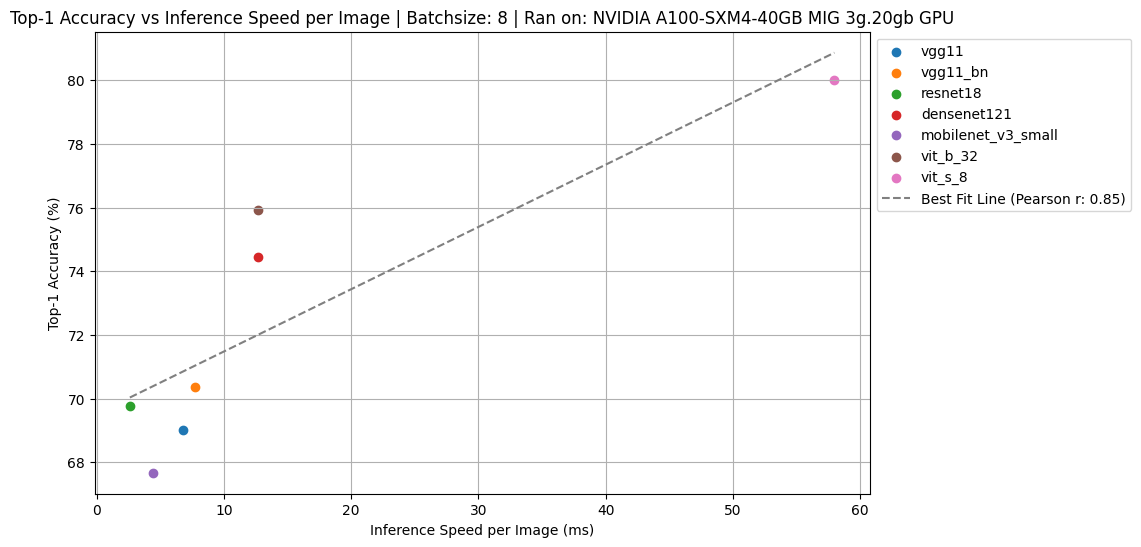
\includegraphics[width=0.75\textwidth]{"imgs/Top1Acc-vs-Inference.png"}
    \caption{Top-1 Accuracy vs Inference Speed per Image}
    \label{fig:Top1Acc-vs-Inference}
\end{figure}

For inference speed against number of trainable parameters, we see no correlation. The number of trainable parameters
should only play a role when the model is being trained, not during inferencing, so this result matches our
expectations. Shown in Figure \ref{fig:NumParams-vs-Inference}.
\begin{figure}[h]
    \centering
    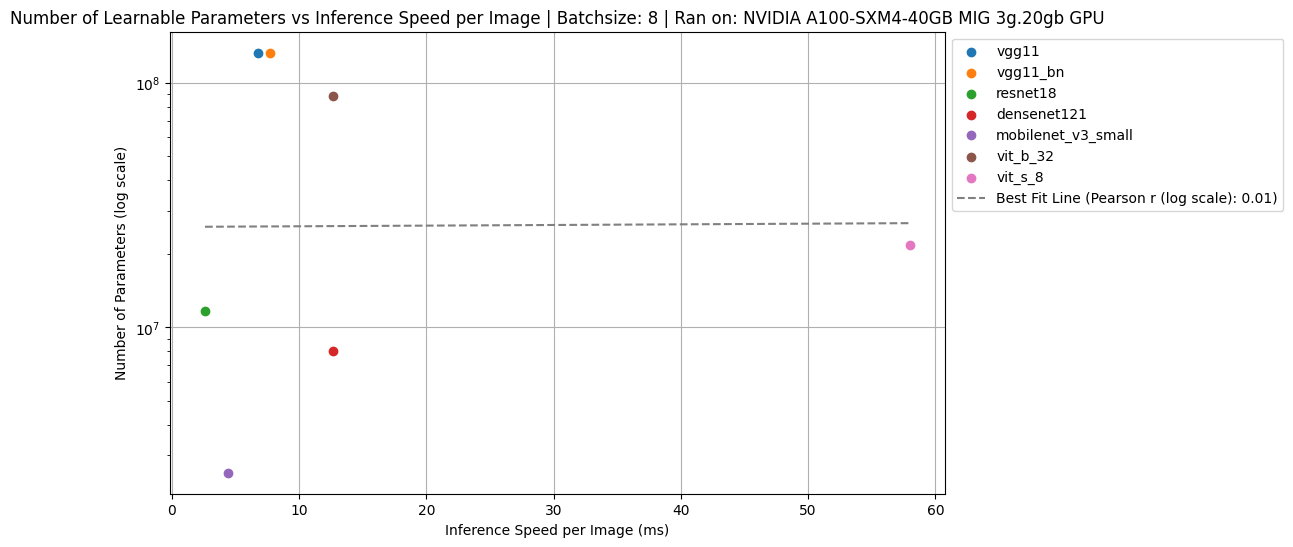
\includegraphics[width=0.75\textwidth]{"imgs/NumParams-vs-Inference.png"}
    \caption{Number of Trainable Parameters vs Inference Speed per Image}
    \label{fig:NumParams-vs-Inference}
\end{figure}

\subsubsection{Inference Speed per Image with and without torch.no\_grad()}
With torch.no\_grad() the inference speed should be faster because gradients are not computed and stored for the
backward pass within the context manager's scope, thus requiring less operations and saving compute. This is
confirmed by the results, the inference speed is slightly faster with torch.no\_grad() across the models. Shown in
Figure \ref{fig:Inference-vs-noGrad}.
\begin{figure}[h]
    \centering
    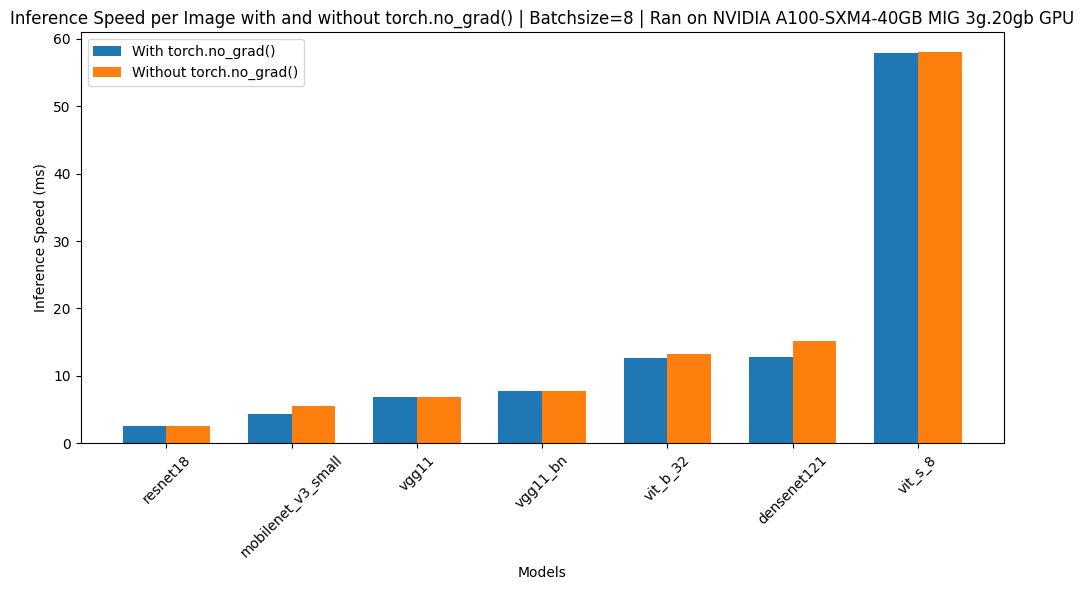
\includegraphics[width=0.75\textwidth]{"imgs/Inference-vs-noGrad.png"}
    \caption{Inference Speed per Image with and without torch.no\_grad()}
    \label{fig:Inference-vs-noGrad}
\end{figure}

\subsubsection{vRAM Usage with and without torch.no\_grad()}
Like with the inference speed, the vRAM usage should be lower with torch.no\_grad() because gradients are not
stored for the backward pass when performing tensor operations, freeing up memory. Much more considerably than the
inference speed, the vRAM usage is lower when using torch.no\_grad() as seen in the plot. Shown in Figure
\ref{fig:VRAM-vs-noGrad}.
\begin{figure}[h]
    \centering
    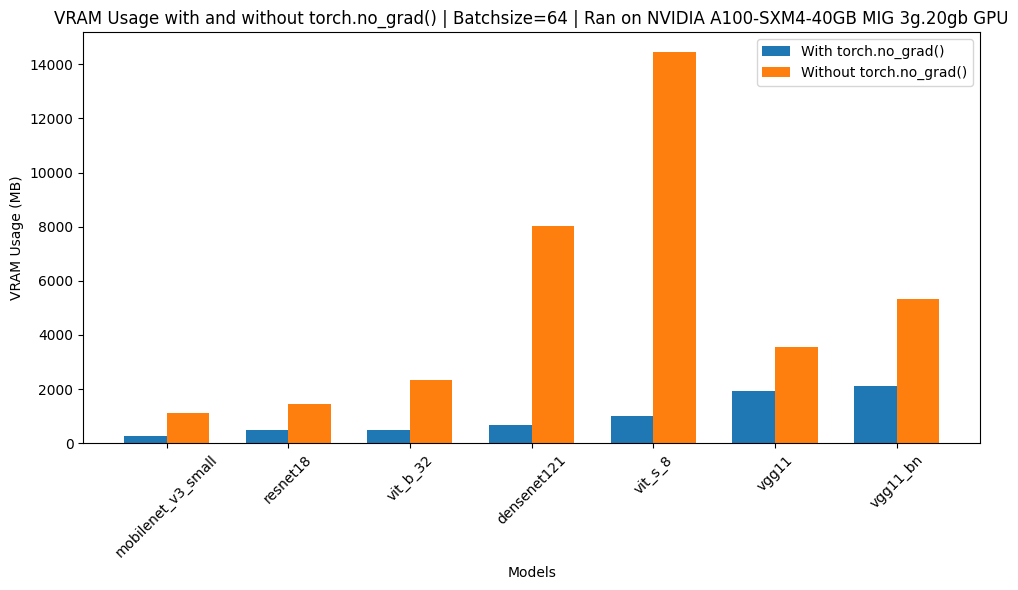
\includegraphics[width=0.75\textwidth]{"imgs/VRAM-vs-noGrad.png"}
    \caption{vRAM Usage with and without torch.no\_grad()}
    \label{fig:VRAM-vs-noGrad}
\end{figure}
\bigskip
% ------------------------------

\subsection{Fine-tuning}
\subsubsection{Retraining ResNet-18's Fully Connected Layer}
Using the specifications and default hyperparameters from the assignment, the retrained model achieved a test
accuracy of 58.55\% in CIFAR-100.

\subsubsection{Increasing Model Performance using Data Augmentation}
By applying \texttt{torchvision.transforms.RandomHorizontalFlip(p=0.5)} around half of the images in the training
set are flipped horizontally. This should increase the model's performance because it is being trained on more
varied data, thus making it more robust to different inputs. The model achieved a test accuracy of 59.27\%, a small
improvement.

\subsubsection{Last vs First Convolutional Layer}
The first convolutional layers tend to capture lower-level features like edges, corners or textures, while the last
layers capture higher-level features like shapes and objects in a larger receptive field. As such, better performance
should be achievable by fine-tuning the last layers (along with the classifier layers) because they are more
specialized to the downstream task than the first layers.
\bigskip
% ==============================

\section{Visual Prompting}
\subsection{CLIP Baseline}
\subsubsection{Top-1 Accuracy on CIFAR-10 and CIFAR-100 with CLIP ViT-B/32 Backbone}
% Zero-shot CLIP top-1 accuracy on cifar10/train: 88.726
% Zero-shot CLIP top-1 accuracy on cifar10/test: 88.94
% Zero-shot CLIP top-1 accuracy on cifar100/train: 63.564
% Zero-shot CLIP top-1 accuracy on cifar100/test: 63.14999999999999
\begin{table}[h]
    \centering
    \begin{tabular}{|l|c|c|}
    \hline
    \rowcolor{Gray}
    \textbf{Dataset} & \textbf{Train Accuracy (\%)} & \textbf{Test Accuracy (\%)} \\ \hline
    CIFAR-10 & 88.73 & 88.94 \\ \hline
    CIFAR-100 & 63.56 & 63.15 \\ \hline
    \end{tabular}
    \caption{Zero-shot CLIP Top-1 Accuracy on CIFAR-10 and CIFAR-100}
    \label{tab:clip_accuracy}
\end{table}


\subsubsection{Prompting CLIP for a New Classification Task}
\textbf{Prompt:} \textit{"This is an image mostly coloured \_\_\_"}\newline
\textbf{Labels:} \textit{"red", "green", "blue"}
\begin{figure}[h]
    \centering
    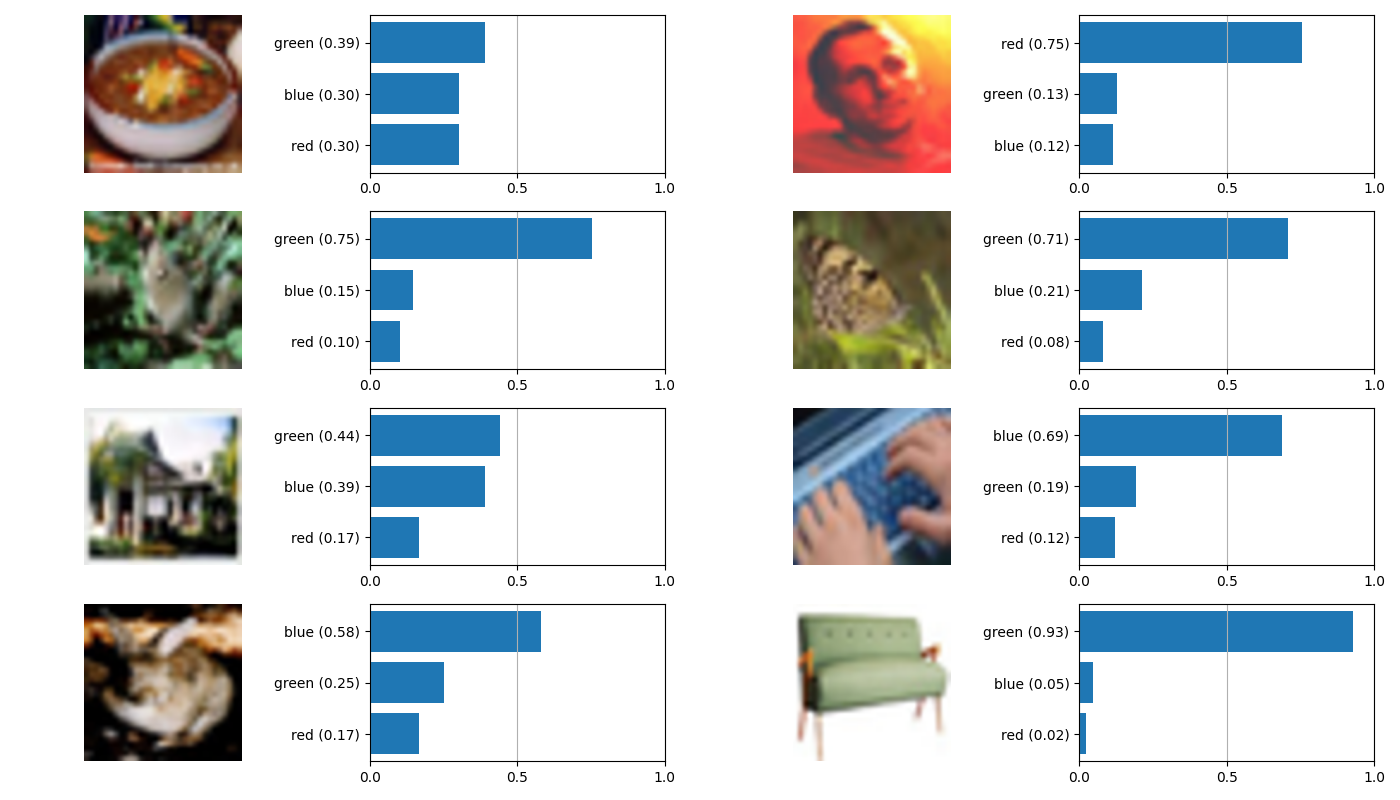
\includegraphics[width=0.75\textwidth]{"imgs/cifar100-test_red,green,blue.png"}
    \caption{Primary Colour Identification}
    \label{fig:CLIP-primary-colour}
\end{figure}

We see in Figure \ref{fig:CLIP-primary-colour} that the model is able to identify the primary colour of the image
with a high degree of accuracy. For images with a distinct primary colour, the model is able to identify it with
high confidence, and for images with no clear distinct primary colour, it returns failry spread out probabilities.
The contrastive learning approach of CLIP allows it to generalize well to new tasks using prompting.
\bigskip

\textbf{Prompt:} \textit{"This image displays an object that is \_\_\_"}\newline
\textbf{Labels:} \textit{"human-made", "from-nature"}
\begin{figure}[h]
    \centering
    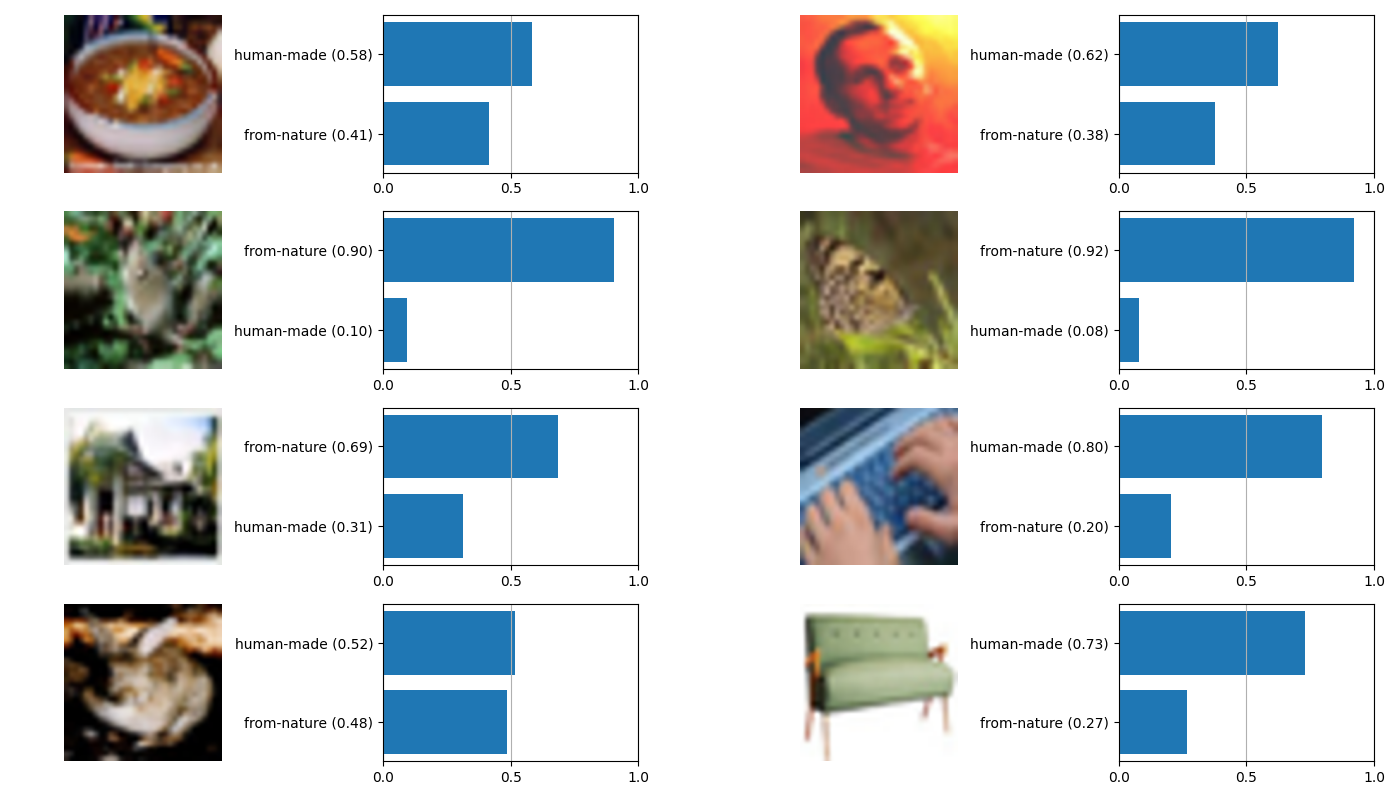
\includegraphics[width=0.75\textwidth]{"imgs/cifar100-test_human-made,from-nature.png"}
    \caption{Distinguishing Human-made and Natural Objects}
    \label{fig:CLIP-human-vs-nature}
\end{figure}

Here too the model performs quite well, considering the task is slightly more abstract than identifying just primary
colours. For clearly human-made objects like a computer keyboard or a couch, the model is able to identify it with
high confidence. It does however mislabel some examples, like the image of the bunny being labelled as human-made. The
more even spread of probabilities for the bunny image suggests that the model is not very confident in its prediction.
See Figure \ref{fig:CLIP-human-vs-nature}.

\bigskip
It therefore seems that CLIP is able to generalize well to new tasks using prompting, but it is not perfect and can
make mistakes when the task is more abstract.
This approach to zero-shot learning is very powerful because it allows us to perform a wide range of tasks without
having to train a new model for each task. This is especially useful when the task is not very complex and does not
require a lot of training data, because training a new model for each task would be very inefficient.
\bigskip

\subsection{Effect of Prompt Types on Classification Accuracy}
\begin{figure}[h]
    \centering
    \begin{minipage}[b]{0.45\textwidth}
        \centering
        
\includegraphics[width=0.8\textwidth]{"imgs/prompt_fixed_patch.png"}
        \caption{Fixed Patch Visual Prompt (Single Pixel Top-Left)}
        \label{fig:prompt-fixed}
    \end{minipage}
    \hfill
    \begin{minipage}[b]{0.45\textwidth}
        \centering
        
\includegraphics[width=0.8\textwidth]{"imgs/prompt_padding.png"}
        \caption{Padding Visual Prompt}
        \label{fig:prompt-padding}
    \end{minipage}
\end{figure}

% CIFAR-10 fixed_patch and prompt size 1 Acc@1 89.570
% CIFAR-10 padding and prompt size 30 Acc@1 92.740
% CIFAR-100 fixed_patch and prompt size 1 Acc@1 64.490
% CIFAR-100 padding and prompt size 30 Acc@1 71.390
\begin{table}[h]
    \centering
    \begin{tabular}{|l|c|c||c|}
    \hline
    \rowcolor{Gray}
    \textbf{Dataset} & \textbf{Fixed Patch Accuracy (\%)} & \textbf{Padding Accuracy (\%)} & \textbf{Baseline Accuracy (\%)} \\ \hline
    CIFAR-10 & 89.57 & 92.74 & 88.94 \\ \hline
    CIFAR-100 & 64.49 & 71.39 & 63.15 \\ \hline
    \end{tabular}
    \caption{CLIP Top-1 Accuracy on CIFAR-10 and CIFAR-100's Test with Different Prompt Types Compared to Baseline}
    \label{tab:clip_accuracy_prompt_types}
\end{table}

Comparing these results obtained using visual prompts on the CIFAR-10 and 100 test set to the baseline results in
seen in Table \ref{tab:clip_accuracy}, we see that the accuracy is higher for both prompt types, with the padding
prompt type performing significantly better than the fixed patch prompt type. This is likely because the padding
prompt type has a lot more trainable parameters (69840 for padding size 30) than the fixed patch prompt type (3 for
patch size 1, one per channel), and thus is able adapt better to the task. Espeically for the CIFAR-100 dataset this
improvement is noticeable. likely due to the fact that the CIFAR-100 dataset is more complex than the CIFAR-10
dataset, and thus requires more trainable parameters to perform well.
\bigskip

\subsection{Deep Prompts}
From Figure 3 in the assignment PDF we see how we can inject a learnable deep prompt into the CLIP model. In the
diagram it is appended to the beginning of the sequence that is fed into a Transformer block. I initially accidentally
appended it to the end of the sequence, but then chose to compare the two approaches which was quite interesting to
see. I also investigated the effect of different numbers of deep prompts (1, 4 \& 8) as well as the injection layer.
The results are shown in Table \ref{tab:clip_accuracy_deep_prompts}, as well as a comparison between the best visual
prompt accuracies and baseline readings in Table \ref{tab:clip_accuracy}.

\begin{table}[h]
    \centering
    \begin{tabular}{|l|c|c|c|c|}
    \hline
    \rowcolor{Gray}
    \textbf{Dataset} & \textbf{Injection Layer} & \textbf{Prompts} & \textbf{Front Acc (\%)} & \textbf{Back Acc (\%)} \\ \hline
    \multirow{9}{*}{CIFAR-10}  
                               & \multirow{3}{*}{0} & 1 & 95.32 & \textbf{95.48} \\ \cline{3-5}
                               &                     & 4 & \textbf{96.31} & 94.97 \\ \cline{3-5}
                               &                     & 8 & \textbf{96.59} & 94.67 \\ \cline{2-5}
                               & \multirow{3}{*}{6} & 1 & 94.63  & \textbf{94.82} \\ \cline{3-5}
                               &                     & 4 & \textbf{95.82} & 94.46 \\ \cline{3-5}
                               &                     & 8 & \textbf{96.00} & 94.23 \\ \cline{2-5}
                               & \multirow{3}{*}{11}& 1 & 91.17  & \textbf{92.44} \\ \cline{3-5}
                               &                     & 4 & 91.18  & \textbf{92.35} \\ \cline{3-5}
                               &                     & 8 & 89.25  & \textbf{92.19} \\ \hline
    \multirow{9}{*}{CIFAR-100} 
                               & \multirow{3}{*}{0} & 1 & 75.90  & \textbf{76.27} \\ \cline{3-5}
                               &                     & 4 & \textbf{78.43} & 75.78 \\ \cline{3-5}
                               &                     & 8 & \textbf{79.98} & 74.86 \\ \cline{2-5}
                               & \multirow{3}{*}{6} & 1 & 73.72  & \textbf{74.29} \\ \cline{3-5}
                               &                     & 4 & \textbf{76.95} & 74.01 \\ \cline{3-5}
                               &                     & 8 & \textbf{78.11} & 73.56 \\ \cline{2-5}
                               & \multirow{3}{*}{11}& 1 & \textbf{69.62} & 68.39 \\ \cline{3-5}
                               &                     & 4 & \textbf{69.61} & 68.00 \\ \cline{3-5}
                               &                     & 8 & \textbf{69.64} & 67.67 \\ \hline
    \end{tabular}
    \caption{Image Classification Performance with CLIP using Different Numbers of Prompts, Injected at Different Layers and Appended to the Front or Back of the Sequence}
    \label{tab:clip_accuracy_deep_prompts}
\end{table}

Injecting prompts at early layers yields higher classification performance across the board than at later layers. This could be because it allows the model to learn more specialized lower-level
features that are more useful for the classification task at hand, although this could differ with dataset too. The
difference between injecting at layer 0 and 6 is also less pronounced than between layer 6 and 11, which might hint to
the fact that deep prompts are most useful for lower-level to mid-level features.
\newline \newline
Increasing the number of prompt generally correlates well with an increase in classification accuracy too, having
the largest effect when injecting at early to middle layers on the CIFAR-100 dataset. This could be because the
CIFAR-100 dataset is more complex than the CIFAR-10 dataset and the model benefits from having more guidance from the
prompts.
\newline \newline
Appending the prompts to the front of the sequence does seem to yield
slightly better results than appending them to the back of the sequence. Although the attention mechanism of the
Transformer should allow the model to learn to attend to the prompts regardless of their position in the sequence,
appending our style of prompt (''This is a photo of a \{\}") perhaps is better suited to being at the beginning,
whereas more of a question or summary style prompt could be better suited to being at the end of the sequence. This
is just specularitory and could be interesting for futher investigation.
\newline \newline
We see that the best performing deep prompt model outperforms the visual prompt model, resulting in a considerable
improvement over the baseline model. 
\begin{table}[h]
    \centering
    \begin{tabular}{|l|c|c|c|}
    \hline
    \rowcolor{Gray}
    \textbf{Dataset} & \textbf{Deep Prompt Acc (\%)} & \textbf{Visual Prompt Acc (\%)} & \textbf{Baseline Acc (\%)} \\ \hline
    CIFAR-10 & 96.59 & 92.74 & 88.94 \\ \hline
    CIFAR-100 & 79.98 & 71.39 & 63.15 \\ \hline
    \end{tabular}
    \caption{CLIP Top-1 Accuracy on CIFAR-10 and CIFAR-100's Test Set with Different Prompt Types Compared to Baseline}
    \label{tab:clip_accuracy}
\end{table}

The reason why deep prompts might outperform the visual prompts is that they can interact with the latent
representation of the image in the model, allowing more complex interactions between the prompt and the image. This
can guide the network better than the visual prompts which only can augment the raw input data.

\subsection{Robustness to Noise}
I investigated how robust CLIP and Resnet-18 are to distributional shifts on CIFAR-100 by adding Gaussian noise to
the test set. The previously trained CLIP model using a visual padding prompt of size 30 was used for this, while
for Resnet-18 the fine-tunned model was used where only the fully connected layer was retrained - but not the one
being shown augmented data during training as to not bias it towards having seen noisy data before.

Previously, in this configuration CLIP achieved a test accuracy of 71.39\% and Resnet-18 achieved a test accuracy
of 58.55\%. The results of adding Gaussian noise to the test set are shown in Table \ref{tab:robustness}.

\begin{table}[h]
    \centering
    \begin{tabular}{|l|c|c|}
    \hline
    \rowcolor{Gray}
    \textbf{Test Dataset} & \textbf{CLIP Accuracy (\%)} & \textbf{Resnet-18 Accuracy (\%)} \\ \hline
    CIFAR-100 & 71.39 & 58.55 \\ \hline
    CIFAR-100 + Gaussian Noise & 61.89 & 25.15 \\ \hline
    \end{tabular}
    \caption{CLIP and Resnet-18 Top-1 Accuracy on CIFAR-100's Test Set with and without Gaussian Noise}
    \label{tab:robustness}
\end{table}

Where we can see a clear drop in accuracy for both models, although CLIP seems much more robust to the noise than
Resnet-18, CLIP lost around 10\% accuracy while Resnet-18's more than halved.
\bigskip

\subsection{Visual Prompts Effectiveness on CIFAR-110}


\end{document}